\section{Introductie}

\subsection{Definitie van Machine Learning}

Machine learning kan gedefinieerd worden met behulp van een quote van Tom Mitchell: 

\begin{quote}
	“A computer program is said to learn from experience E with respect to some class of tasks T and performance measure P, if its performance at tasks in T, as measured by P, improves with experience E.” — Tom Mitchell, Professor at Carnegie Mellon University, 1998. 
\end{quote}

\noindent
Het komt er dus op neer dat machine learning een proces  is waarbij een computerprogramma leert van ervaring. Er bestaan een aantal verschillende algoritmes binnen machine learning. Zo is er onder andere \textit{supervised learning}, \textit{unsupervised learning} en zijn er \textit{recommender systems}. \\
\newline
Bij \textit{supervised learning} krijgt het model de data en de correcte labels en zal het op basis daarvan voor nieuwe data de output proberen te voorspellen. We kunnen binnen \textit{supervised learning} verder onderscheid maken tussen regressie-problemen waarbij we een continue output-waarde proberen te voorspellen en een classificatie-probleem waarbij we een discrete output-waarde zullen hebben (0 of 1). \\
\newline
Bij \textit{unsupervised learning} krijgt het model enkel de data en zal het de datapunten clusteren op basis van de afstand ertussen. Figuur \ref{fig:supervised-vs-unsupervised-learning} toont het verschil tussen \textit{supervised} en \textit{unsupervised learning}.

\begin{figure}[h]
	\centering
	\begin{subfigure}{.5\textwidth}
		\centering
		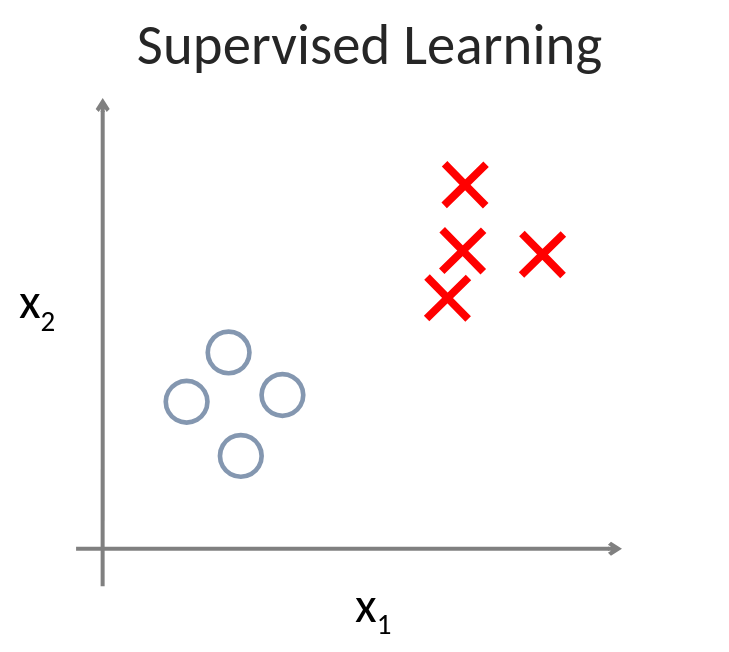
\includegraphics[height=0.45\textwidth]{images/1-supervised-learning.png}
		\caption{Supervised learning}
		\label{fig:supervised-learning}
	\end{subfigure}%
	\begin{subfigure}{.5\textwidth}
		\centering
		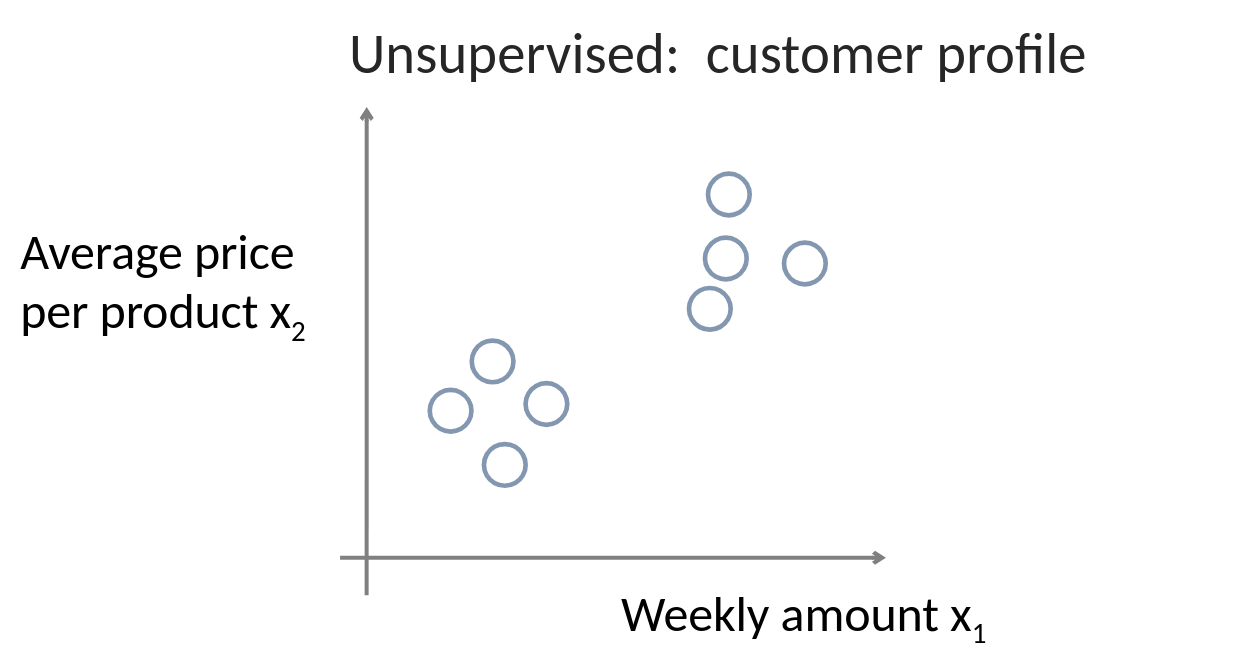
\includegraphics[height=0.45\textwidth]{images/2-unsupervised-learning.png}
		\caption{Unsupervised learning}
		\label{fig:unsupervised-learning}
	\end{subfigure}
	\caption{Verschil tussen \textit{supervised} en \textit{unsupervised learning}}
	\label{fig:supervised-vs-unsupervised-learning}
\end{figure}

\noindent
\textit{Recommender systems} zijn algoritmes die relevante zaken aanbevelen aan gebruikers. Dit draagt bij aan de ervaring van de gebruiker omdat hij gepersonaliseerde suggesties krijgt en wordt veel gebruikt bij online shopping, streamingdiensten en sociale media. De hoofdonderdelen van deze algoritmes zijn het profiel van de gebruiker en van de items.

\subsection{Etisch aspect van Machine Learning en AI}

Wanneer we kijken naar machine learning en AI, zijn er enkele etische aspecten waar we rekening mee moeten houden. Zo kan de data die we gebruiken een bepaalde bias met zich mee brengen. Een voorbeeld hiervan is wanneer we een model om borstkanker op een visuele manier te detecteren enkel zouden trainen met afbeeldingen van witte mensen. Het gevolg hiervan zou zijn dat het model niet zal werken voor mensen met een zwarte huidskleur. Daarnaast moeten we ook in de gaten houden of het doel waarvoor we ons model willen gebruiken wel etisch is. 
